\documentclass[12pt,fleqn]{article}\usepackage{../../common}
\begin{document}
Filtrelemek

\inputminted[fontsize=\footnotesize]{python}{filt.py}

\begin{minted}[fontsize=\footnotesize]{python}
import filt
fy=300; #signal frequency in Hz
wy=2*np.pi*fy; #signal frequency in rad/s
fs=50; #sampling frequency in Hz
tiv=1./fs; #time interval between samples;
tend = 5 # seconds
t=np.linspace(0,tend,tend/tiv); #time intervals set (5 seconds)

y=0.6*np.sin(wy*t)+0.3*np.sin(3*wy*t)+0.2*np.sin(5*wy*t); #signal data set
f=plt.figure()
plt.plot(t,y)
plt.savefig('tser_freq_05.png')

fou = np.fft.fft(y, fs)
hmag=np.real(fou); ah=hmag/len(t);
f=plt.figure()
plt.stem(range(10),ah[:10])
plt.savefig('tser_freq_06.png')

order = 32
fc1 = 2
fs = 20
f1 = filt.sinc_filter_low(order, fc1, fs).T[0];

y1 = np.convolve(f1, y)
f=plt.figure()
plt.plot(np.arange(len(y1)), y1)
plt.savefig('tser_freq_08.png')

fou = np.fft.fft(y1, fs)
hmag=np.real(fou); ah=hmag/len(t);
f=plt.figure()
plt.stem(range(10),ah[:10])
plt.savefig('tser_freq_07.png')
\end{minted}

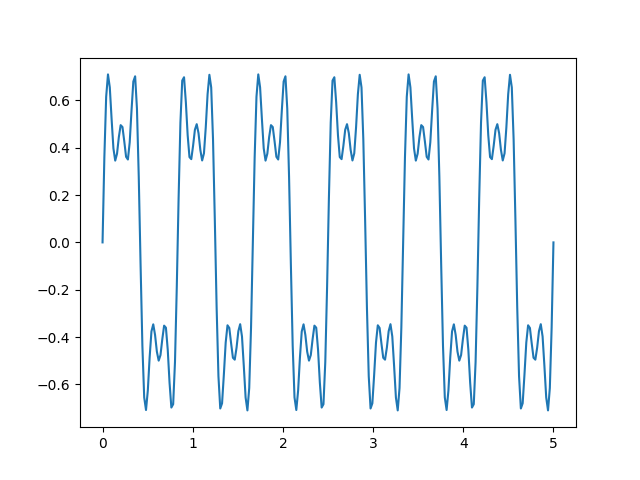
\includegraphics[width=20em]{tser_freq_05.png}

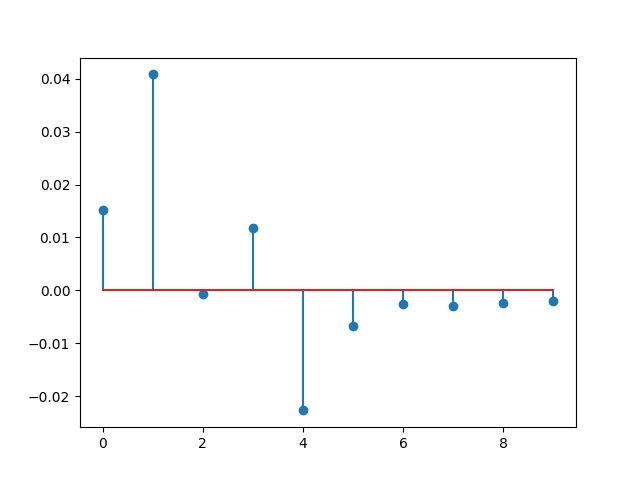
\includegraphics[width=20em]{tser_freq_06.png}

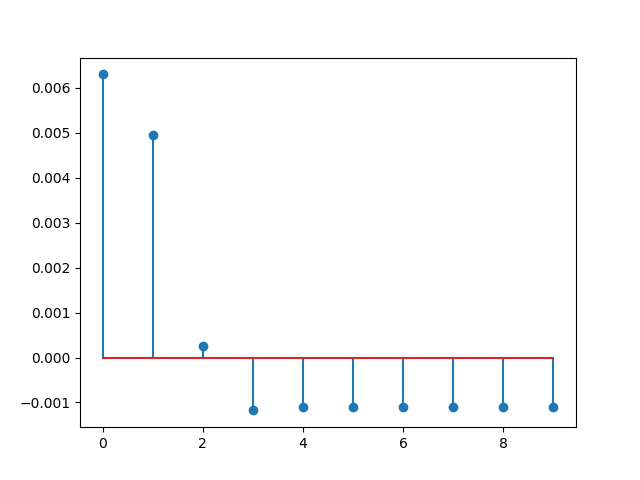
\includegraphics[width=20em]{tser_freq_07.png}

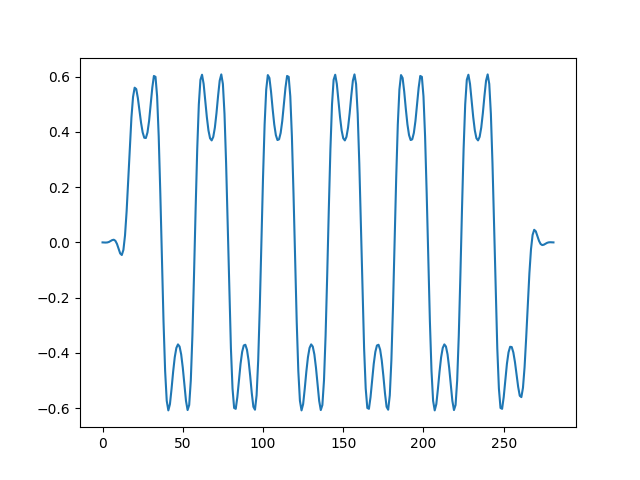
\includegraphics[width=20em]{tser_freq_08.png}


\begin{minted}[fontsize=\footnotesize]{python}
fc1 = 3
f2 = filt.sinc_filter_high(order, fc1, fs).T[0];

y2 = np.convolve(f2, y)
f=plt.figure()
plt.plot(np.arange(len(y2)), y2)
plt.savefig('tser_freq_10.png')

fou = np.fft.fft(y2, fs)
hmag=np.real(fou); ah=hmag/len(t);
f=plt.figure()
plt.stem(range(10),ah[:10])
plt.savefig('tser_freq_09.png')
\end{minted}

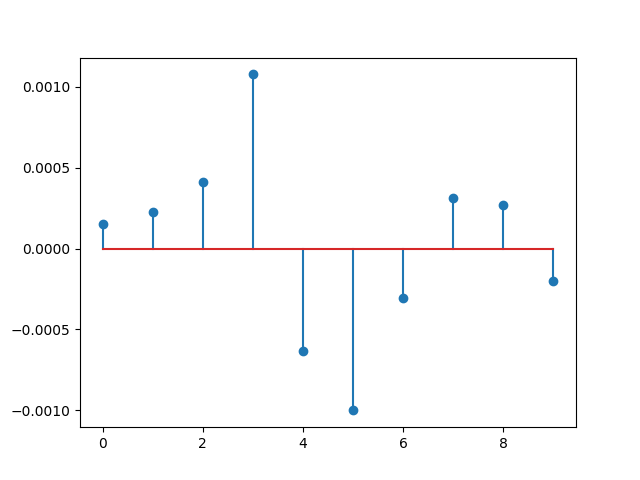
\includegraphics[width=20em]{tser_freq_09.png}

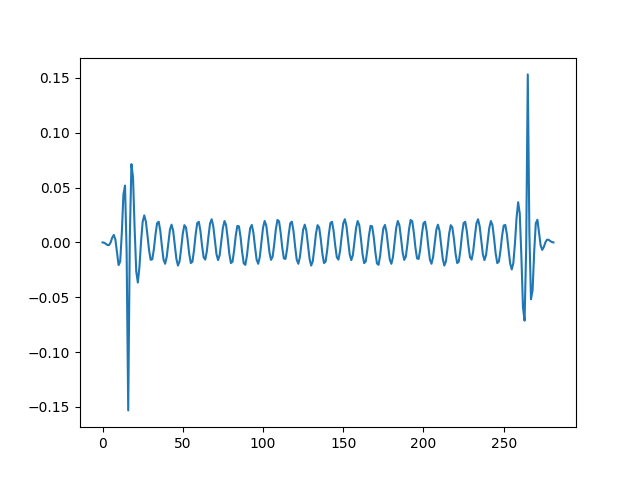
\includegraphics[width=20em]{tser_freq_10.png}


\begin{minted}[fontsize=\footnotesize]{python}
fc1 = 2
fc2 = 4
f3 = filt.sinc_filter_band(order, fc1, fc2, fs);

y3 = np.convolve(f3, y)
f=plt.figure()
plt.plot(np.arange(len(y3)), y3)
plt.savefig('tser_freq_12.png')

fou = np.fft.fft(y3, fs)
hmag=np.real(fou); ah=hmag/len(t);
f=plt.figure()
plt.stem(range(10),ah[:10])
plt.savefig('tser_freq_11.png')
\end{minted}

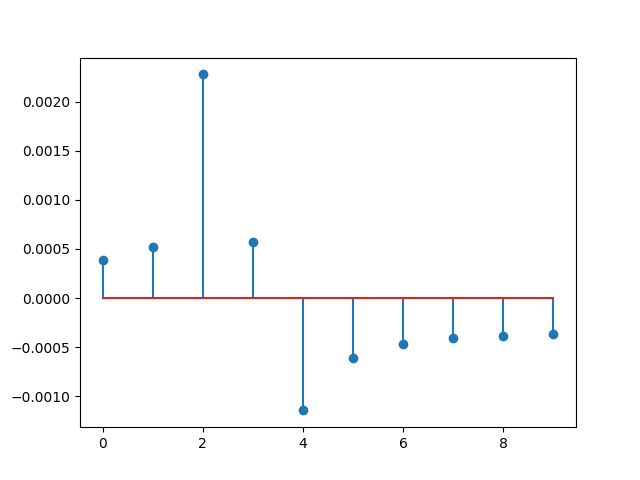
\includegraphics[width=20em]{tser_freq_11.png}

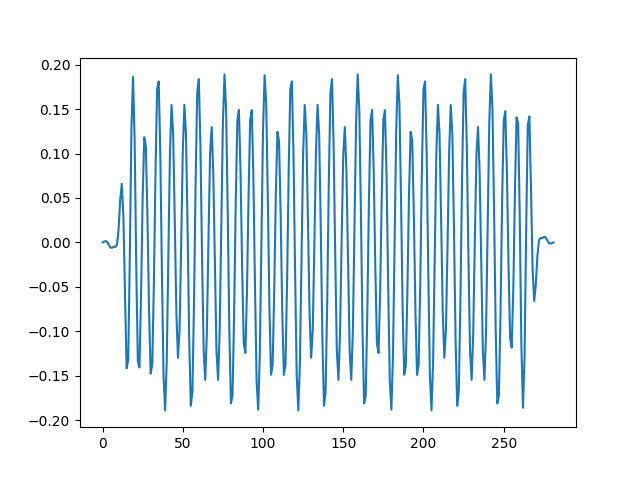
\includegraphics[width=20em]{tser_freq_12.png}


\begin{minted}[fontsize=\footnotesize]{python}
from scipy.signal import butter, lfilter
def butter_bandpass(lowcut, highcut, fs, order=5):
    nyq = 0.5 * fs
    low = lowcut / nyq
    high = highcut / nyq
    print  low, high
    b, a = butter(order, [low, high], btype='band')
    return b, a

def butter_bandpass_filter(data, lowcut, highcut, fs, order=5):
    b, a = butter_bandpass(lowcut, highcut, fs, order=order)
    y = lfilter(b, a, data)
    return y

yb = butter_bandpass_filter(y, 2, 4, fs, order=5)
plt.plot(np.arange(len(yb)), yb)
plt.savefig('tser_freq_13.png')
\end{minted}

\begin{verbatim}
0.2 0.4
\end{verbatim}

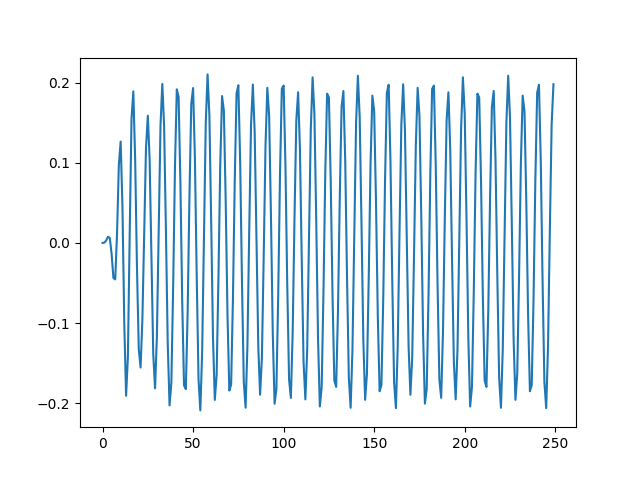
\includegraphics[width=20em]{tser_freq_13.png}








[devam edecek]

Kaynaklar

\end{document}






















